% !TeX spellcheck = en_US
% !TeX encoding = UTF-8
% !TeX root = ../thesis.tex

\chapter{Recursive Surrogate-Modeling for MORE}
In this chapter we will first motivate the idea of recursively
estimating the surrogate model for the MORE algorithm.
We formulate the surrogate model estimation
as a regression problem and present our solution.
Then we combine our approach with the MORE algorithm
Finally we discuss various data preprocessing techniques.

\section{Surrogate Model Estimation}

\subsection{Motivation}
So far, the surrogate model has been estimated from scratch in each
iteration using samples and corresponding
values of the objective function. 
However, subsequent models are correlated
due to the locality of the data (see figure
(TODO: add Figure of surrogate model)).
This arises from the fact that the KL-divergence is
used to bound the distance between
subsequent search distributions. Therefore recursive estimation
techniques may be able to utilize the information of previous
surrogate models and thus reduce the total amount of samples needed.
Additionally this may also reduce the runtime of the algorithm.

The surrogate model is a of the form
\begin{align}
  \label{surrogate}
  \mathcal{R}(\mathbf{x}) = -\frac{1}{2} \mathbf{x}^T \mathbf{R} \mathbf{x}
  + \mathbf{x}^T \mathbf{r} + r 
\end{align}
With a quadratic term $\mathbf{R} \in \mathbb{R}^{n \times n}$,
a linear term $\mathbf{r} \in \mathbb{R}^{n}$ and a scalar $r$,
here $n$ denotes the dimension of the objective function.
Using a quadratic model is sufficient as the exponential of the
Gaussian is also quadratic in the parameters.
A more complex model could not be exploited by
a Gaussian distribution \citep{abdolmaleki2015model}.


% TODO: include 2D contour line or 3d version of subsequent models

\subsection{Regression Problem}
We formulate the surrogate estimation task as
a regression problem (\ref{eq:regression}) by using
a feature function $\phi(\mathbf{x})$ which returns
a bias term, all linear and all quadratic terms. The dimensionality of
$\phi(\mathbf{x})$ is $D = 1 + d + d(d + 1) / 2$, where $d$
is the dimensionality of the parameter space.
\begin{align}
  \label{eq:regression}
  y = \phi(\mathbf{x}) \beta + \epsilon
\end{align}
% The surrogate model parameters are in $\beta$
% a vector of length $D$ containing first the
% scaler than $d$ linear terms and then $d(d+1) /2$ quadratic terms
% (the lower triangular matrix).
Our data are the samples and corresponding objective function
values $\mathcal{D} = \{(\mathbf{x}_1, y_1),...,(\mathbf{x}_n, y_n)\}$.
To solve the regression problem we set up
the design matrix $\mathbf{X}$ as depicted in \cref{eq:lgs}.
One row $\mathbf{X}_{k}$ first contains a one for the bias term.
Then the next $d$ entries are made up of the corresponding
sample $\mathbf{x}_k$ for the linear term.
The final $d(d + 1) / 2$  entries are
the lower triangular matrix of the product $\mathbf{x}_k \mathbf{x}_k^T$,
which we denote by tril$(\mathbf{x}_k \mathbf{x}_k^T)$.
% Corresponding to the set
% $\text{tri}(\mathbf{x}) = \{x_1^2 , x_1 x_2 , x_1 x_3 ,
% \cdots , x_2^2 , x_2 x_3 \cdots\}$,
% where we multiply each sample entry with itself and all entries with
% higher index. 

For the least squares (LS) approach with $n \geq D$ samples
we get the following system of linear equations. 
\begin{equation}
  \label{eq:lgs}
\begin{bmatrix} y_1 \\ y_2 \\ \vdots \\ y_n \end{bmatrix}
=
\underbrace{
\begin{bmatrix}
  1 & \mathbf{x}_1 & \text{tril}(\mathbf{x}_1 \mathbf{x}_1^T) \\
  1 & \mathbf{x}_2 & \text{tril}(\mathbf{x}_2 \mathbf{x}_2^T) \\
  \vdots & \vdots & \vdots \\
  1 & \mathbf{x}_n & \text{tril}(\mathbf{x}_n \mathbf{x}_n^T) \\
\end{bmatrix}}_{\mathbf{X}}
\begin{bmatrix}
  \beta_1 \\ \beta_2 \\ \vdots \\ \beta_D
\end{bmatrix}
+
\begin{bmatrix}
  \epsilon_1 \\
  \epsilon_2 \\
  \vdots \\
  \epsilon_n
\end{bmatrix}
\end{equation}

This can be solved with ordinary least squares
$\beta = (\mathbf{X}^T \mathbf{X})^{-1} \mathbf{X} \mathbf{y}$.
For our experiments we use a form of ridge regression \citep{hoerl1975ridge}.


The solution vector $\beta$ contains the surrogate model parameters
$(r, \mathbf{r}, \mathbf{R})$. We also assume that
the measurement noise $\epsilon_k$ is zero mean Gaussian
$\epsilon_k \sim N(0, \sigma^2)$ distributed.


Using recursive estimation we
can process each pair of samples and rewards $(\mathbf{x}_k, y_k)$ one
at a time.
$$
 y_k =
 \big(1 \;  \mathbf{x}_k \; \text{tril}(\mathbf{x}_k \mathbf{x}_k^T) \big)
\begin{pmatrix}
  \beta_1 \\ \beta_2 \\ \vdots \\ \beta_D
\end{pmatrix} 
+ \epsilon_k
$$

\section{Recursive Least Squares}
Let us now show how we use the recursive least squares approach
to compute the solution vector $\beta$ to the regression problem.

We did not find a good state transition model for our problem of
estimating the parameters of the quadratic model of the objective function.
We tried some momentum based approaches during our evaluation but
did not receive any promising results. Therefore we limit our approach to
adding model noise in the prediction step and
using an Identity matrix as the state transition matrix $\mathbf{A}$.

We want to compute
$$ p(\beta_k | y_{1:k-1}, \mathbf{x}_{1:k-1}) = \text{N}(\beta_k | m_k, P_k) $$

Our prior $m_0$ is chosen such that for the
first surrogate model parameters
we set the quadratic term to an identity matrix $\mathbf{R} = \mathbf{I}$
and the other terms to zero $ \mathbf{r} = \mathbf{0}$ and $ r = 0$.
The covariance matrix is initialized as  $P_0 = \delta \mathbf{I}$ with
the parameter $\delta$ controlling how confident
we are in our prior. By limiting the prediction step of the Kalman Filter
\cref{KF_prediction} to adding model noise we get the basic
version of Recursive Least squares \Cref{RLS:basic} with a drift model for the
parameters to be estimated.

\begin{algorithm}[H]
\SetKw{KwInit}{Initialization:}
\DontPrintSemicolon
\SetAlgoLined

\KwIn{$\{(\mathbf{x}_1,y_1),\cdots,(\mathbf{x}_N,y_N)\}$
  stream of samples and rewards, \\
  $Q$ model noise, $\sigma^2$ measurement noise}
\KwInit{$\mathbf{m}_0$,  $\mathbf{P}_0 = \delta \mathbf{I}$}

\For{$n = 1,...,N$}
{
  $\mathbf{P}_n^- = \mathbf{P}_{n-1} + Q$ \;
  $~$ \;
  \Begin(Update Step)
  {
    $S_n = \phi(\mathbf{x}_n) \mathbf{P}_n^- \phi(\mathbf{x}_n)^T + \sigma^2$ \;
    $\textbf{K}_n = \textbf{P}_{n}^{-} \textbf{H}^T_n S_n^{-1}$ \;
    $\textbf{m}_n = \textbf{m}_{n-1} + \textbf{K}_n [y_n - \textbf{H}_n \textbf{m}_{n-1}]$ \;
    $\textbf{P}_n = \textbf{P}_{n}^{-} - \textbf{K}_n S_n \textbf{K}_n^T $ \;
  }
}
\caption{Recursive Least squares with Drift Model}
\label{RLS:basic}
\end{algorithm}


\section{Data Preprocessing Techniques}
To improve the performance of the algorithm we examined several
data processing techniques. Some key challenges
that arise in the data  are
high range of objective values,
and dealing with sharp bumps in reward from
penalties (e.g collisions).

\subsection{Whitening}
Whitening is a common data preprocessing method in statistical analysis
to transform a correlated random vector into an uncorrelated one
\citep{kessy2018optimal}.
We employ whitening to our algorithm, to reduce the complexity of the
parameters to be estimated. 

\textit{Whitening} is a linear transformation that converts a $d$-dimensional
random vector $\mathbf{x} = (x_1,...,x_d)^T$ with mean
$\text{E}(\mathbf{x}) = \mathbf{\mu} = (\mu_1,...,\mu_d)^T$ and
positive definite $d \times d$ covariance matrix
var$(\mathbf{x}) = \Sigma$ into a new random vector
\begin{align}
  \label{whitening}
 \mathbf{z} = (z_1,...,z_d)^T = \mathbf{W}\mathbf{x}
\end{align}

of the same dimension $d$ and with unit diagonal ``white'' covariance
var$(\mathbf{z}) = \mathbf{I}$. The square $d \times d$
matrix $\mathbf{W}$ is called the whitening matrix.

The whitening transformation defined in Equation \Cref{whitening} requires
the choice of a suitable whitening matrix $W$.
Since $\text{var}(z) = \mathbf{I}$ it follows that
$\mathbf{W}\Sigma \mathbf{W}^T = \mathbf{I}$ and thus
$\mathbf{W}(\Sigma \mathbf{W}^T\mathbf{W}) = \mathbf{W}$, which
is fulfilled if $\mathbf{W}$ satisfies the condition
$$ \mathbf{W}^T \mathbf{W} = \Sigma^{-1} $$
This constrain does not uniquely determine the whitening
matrix $\mathbf{W}$, instead given $\Sigma$ there are infinitely many
possible matrices $\mathbf{W}$, because it allows for rotational freedom.

We used \textit{Cholesky whitening} which is based on
Cholesky factorization of the precision matrix
$\mathbf{L}\mathbf{L}^T = \Sigma^{-1}$, which leads to the whitening
matrix $\mathbf{W}^{\text{Chol}} = \mathbf{L}^T$.
If the cholesky whitening is unsuccessful due to numerical problems,
we instead standardize
the random vector meaning $\text{var}(\mathbf{z}) = 1$ but the correlations
are not removed. In \cref{fig:whitening} we provide an example on using
whitening for our parameter estimation task.

\begin{figure}[t]
  \centering
  \subfigure[][without whitening]{% This file was created by tikzplotlib v0.9.8.
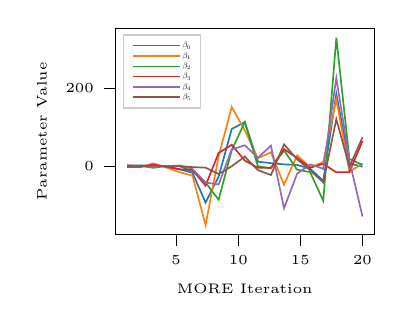
\begin{tikzpicture}

\definecolor{color0}{rgb}{0.12156862745098,0.466666666666667,0.705882352941177}
\definecolor{color1}{rgb}{1,0.498039215686275,0.0549019607843137}
\definecolor{color2}{rgb}{0.172549019607843,0.627450980392157,0.172549019607843}
\definecolor{color3}{rgb}{0.83921568627451,0.152941176470588,0.156862745098039}
\definecolor{color4}{rgb}{0.580392156862745,0.403921568627451,0.741176470588235}
\definecolor{color5}{rgb}{0.549019607843137,0.337254901960784,0.294117647058824}

\begin{axis}[
legend cell align={left},
legend style={
  fill opacity=0.8,
  draw opacity=1,
  text opacity=1,
  at={(0.03,0.97)},
  anchor=north west,
  draw=white!80!black,
  nodes={scale=0.3, transform shape}
},
height=4.2cm,
tick align=outside,
tick pos=left,
% title={LS without whitening},
x grid style={white!69.0196078431373!black},
xmin=0.105263157894737, xmax=20.9473684210526,
ticklabel style = {font=\tiny},
xlabel={\tiny MORE Iteration},
ylabel={\tiny Parameter Value},
% ylabel={\tiny parameter value},
xtick style={color=black},
y grid style={white!69.0196078431373!black},
ymin=-174.244763415887, ymax=351.999761924147,
ytick style={color=black}
]
\addplot [semithick, color0]
table {%
1.05263157894737 1.06132294723888
2.10526315789474 2.06193739819695
3.15789473684211 1.88073583639135
4.21052631578947 -0.123086283009553
5.26315789473684 -8.07620858630262
6.31578947368421 -17.0593030252393
7.36842105263158 -92.9590241843598
8.42105263157895 -26.8587655640602
9.47368421052632 94.8727821397715
10.5263157894737 112.337829573446
11.5789473684211 11.3159172204001
12.6315789473684 7.71762523100675
13.6842105263158 4.45397090742156
14.7368421052632 3.24803643790387
15.7894736842105 -6.60928495432862
16.8421052631579 -37.4795104545709
17.8947368421053 184.451583940082
18.9473684210526 6.99068247604825
20 -1.46585415702719
};
\addlegendentry{$\beta_0$}
\addplot [semithick, color1]
table {%
1.05263157894737 -0.992314117620414
2.10526315789474 -3.01314990774327
3.15789473684211 6.97978246084472
4.21052631578947 -3.46686242249737
5.26315789473684 -15.4385195628296
6.31578947368421 -24.3729399328898
7.36842105263158 -150.324557718613
8.42105263157895 25.4131163178181
9.47368421052632 151.074877150159
10.5263157894737 91.1106450835075
11.5789473684211 20.0637656430311
12.6315789473684 35.3286957225948
13.6842105263158 -47.4852217976283
14.7368421052632 27.7291797336638
15.7894736842105 -2.61087907632418
16.8421052631579 9.8894259773416
17.8947368421053 170.190330132015
18.9473684210526 -14.3804825527134
20 6.50748273849673
};
\addlegendentry{$\beta_1$}
\addplot [semithick, color2]
table {%
1.05263157894737 -2.08306644308438
2.10526315789474 1.33198284531538
3.15789473684211 -4.47590681832019
4.21052631578947 0.728904102890318
5.26315789473684 -0.0242990789144503
6.31578947368421 -13.0927089261868
7.36842105263158 -41.9204495461011
8.42105263157895 -85.6875477618256
9.47368421052632 40.456690037803
10.5263157894737 112.604643253298
11.5789473684211 -0.374250642973178
12.6315789473684 -5.50737080018894
13.6842105263158 40.0710740662349
14.7368421052632 -8.89380033218496
15.7894736842105 -15.3517937773791
16.8421052631579 -88.643722455558
17.8947368421053 328.079556226873
18.9473684210526 18.6863324064035
20 2.86476720653156
};
\addlegendentry{$\beta_2$}
\addplot [semithick, color3]
table {%
1.05263157894737 -1.36618523255821
2.10526315789474 -1.75164609748179
3.15789473684211 3.97756598366229
4.21052631578947 -1.59815536737886
5.26315789473684 -7.98327909179604
6.31578947368421 -9.76539674526244
7.36842105263158 -49.8840839358279
8.42105263157895 33.6375186411652
9.47368421052632 54.4676472894814
10.5263157894737 14.1860483339669
11.5789473684211 -4.01373690738072
12.6315789473684 -4.12863095342328
13.6842105263158 43.3396258637119
14.7368421052632 20.8801779554118
15.7894736842105 -4.18439075502474
16.8421052631579 6.03093788274091
17.8947368421053 -15.7779315076167
18.9473684210526 -15.4260914382804
20 64.1022103374432
};
\addlegendentry{$\beta_3$}
\addplot [semithick, color4]
table {%
1.05263157894737 2.75266552177
2.10526315789474 0.222631082597896
3.15789473684211 -2.66831225317667
4.21052631578947 -0.157081613253339
5.26315789473684 1.74717757967663
6.31578947368421 -7.03076201430117
7.36842105263158 -41.8997254744993
8.42105263157895 -46.7119714649756
9.47368421052632 42.7112959678472
10.5263157894737 53.1938851548008
11.5789473684211 21.4427472965738
12.6315789473684 52.1938391026262
13.6842105263158 -107.554680884685
14.7368421052632 -19.360791728667
15.7894736842105 4.40529333804277
16.8421052631579 -6.78082110704009
17.8947368421053 224.683079683236
18.9473684210526 14.5493471624127
20 -128.444231803502
};
\addlegendentry{$\beta_4$}
\addplot [semithick, color5]
table {%
1.05263157894737 0.409511212005853
2.10526315789474 -0.0998236829556997
3.15789473684211 0.971438641190439
4.21052631578947 -0.250106429020075
5.26315789473684 0.125506587151471
6.31578947368421 -2.47985362888567
7.36842105263158 -3.94108254673754
8.42105263157895 -20.142947018678
9.47368421052632 -0.266294632024777
10.5263157894737 24.1889734159118
11.5789473684211 -10.1386377753676
12.6315789473684 -22.5649113623647
13.6842105263158 55.7345330983559
14.7368421052632 17.5673205505403
15.7894736842105 -10.6102233927423
16.8421052631579 -41.5055080723722
17.8947368421053 119.908371910163
18.9473684210526 -1.67449071311621
20 72.9632198348565
};
\addlegendentry{$\beta_5$}
\end{axis}

\end{tikzpicture}
}
  \subfigure[][in whitened space]{% This file was created by tikzplotlib v0.9.8.
% \tikzset{export as png}
% \tikzsetnextfilename{ls_whitening}
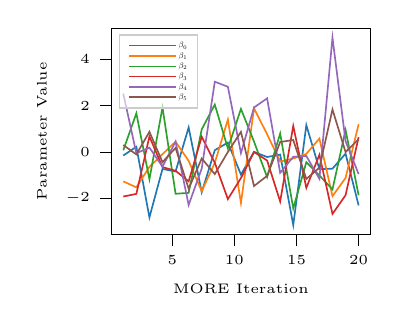
\begin{tikzpicture}

\definecolor{color0}{rgb}{0.12156862745098,0.466666666666667,0.705882352941177}
\definecolor{color1}{rgb}{1,0.498039215686275,0.0549019607843137}
\definecolor{color2}{rgb}{0.172549019607843,0.627450980392157,0.172549019607843}
\definecolor{color3}{rgb}{0.83921568627451,0.152941176470588,0.156862745098039}
\definecolor{color4}{rgb}{0.580392156862745,0.403921568627451,0.741176470588235}
\definecolor{color5}{rgb}{0.549019607843137,0.337254901960784,0.294117647058824}

\begin{axis}[
legend cell align={left},
legend style={
  fill opacity=0.6,
  draw opacity=1,
  at={(0.03,0.97)},
  anchor=north west,  
  text opacity=1,
  draw=white!80!black,
  nodes={scale=0.3, transform shape}
},
tick align=outside,
tick pos=left,
height=4.2cm,
% title={LS with whitening},
ticklabel style = {font=\tiny},
xlabel={\tiny MORE Iteration},
ylabel={\tiny Parameter Value},
% ylabel={\tiny parameter value},
x grid style={white!69.0196078431373!black},
xmin=0.105263157894737, xmax=20.9473684210526,
xtick style={color=black},
y grid style={white!69.0196078431373!black},
ymin=-3.57819481020406, ymax=5.35344627006671,
ytick style={color=black}
]
\addplot [semithick, color0]
table {%
0 nan
1.05263157894737 -0.160438320555973
2.10526315789474 0.219394431243121
3.15789473684211 -2.84098876186452
4.21052631578947 -0.740986055193629
5.26315789473684 -0.853842235649135
6.31578947368421 1.05615797377004
7.36842105263158 -1.75088534391913
8.42105263157895 0.0705918511919139
9.47368421052632 0.39885721031611
10.5263157894737 -0.985345317554263
11.5789473684211 -0.0033406902911266
12.6315789473684 -0.224957401819763
13.6842105263158 -0.120419167449998
14.7368421052632 -3.17221112473721
15.7894736842105 1.15539865077186
16.8421052631579 -0.754182051172667
17.8947368421053 -0.729231023480617
18.9473684210526 -0.0794049070163831
20 -2.32341098853369
};
\addlegendentry{$\beta_0$}
\addplot [semithick, color1]
table {%
0 nan
1.05263157894737 -1.28058969946539
2.10526315789474 -1.53894029689766
3.15789473684211 -0.652695053173459
4.21052631578947 -0.101416098811437
5.26315789473684 0.437679381326199
6.31578947368421 -0.392056022173255
7.36842105263158 -1.70729050930151
8.42105263157895 -0.476763733954958
9.47368421052632 1.39561543789549
10.5263157894737 -2.21966183479818
11.5789473684211 1.88405525337713
12.6315789473684 0.761227631336313
13.6842105263158 -0.422157877808453
14.7368421052632 -0.291442677505589
15.7894736842105 -0.0880591967377688
16.8421052631579 0.573779351363158
17.8947368421053 -1.92031146175774
18.9473684210526 -1.13217123636562
20 1.19487999215437
};
\addlegendentry{$\beta_1$}
\addplot [semithick, color2]
table {%
0 nan
1.05263157894737 0.0650603990168259
2.10526315789474 1.66692307063607
3.15789473684211 -1.19013494700324
4.21052631578947 1.92192393450495
5.26315789473684 -1.81790644534041
6.31578947368421 -1.7780930301196
7.36842105263158 0.97333460454307
8.42105263157895 2.04647534228064
9.47368421052632 0.147437818072115
10.5263157894737 1.85690654709276
11.5789473684211 0.442900159531855
12.6315789473684 -1.096945940621
13.6842105263158 0.792805164400043
14.7368421052632 -2.45161740139127
15.7894736842105 -0.44835764800036
16.8421052631579 -1.0240960807429
17.8947368421053 -1.62856319883405
18.9473684210526 0.944832473104255
20 -1.88201701337283
};
\addlegendentry{$\beta_2$}
\addplot [semithick, color3]
table {%
0 nan
1.05263157894737 -1.93676300196824
2.10526315789474 -1.82257741267246
3.15789473684211 0.663333160936527
4.21052631578947 -0.663275768747337
5.26315789473684 -0.821019212045277
6.31578947368421 -1.28113429602388
7.36842105263158 0.65291281010551
8.42105263157895 -0.472624631498625
9.47368421052632 -2.04993917968636
10.5263157894737 -1.13551165377693
11.5789473684211 -0.00633352819135336
12.6315789473684 -0.376128404445014
13.6842105263158 -2.14995102256074
14.7368421052632 1.12067150617028
15.7894736842105 -1.56239905578431
16.8421052631579 -0.127546346525872
17.8947368421053 -2.69078125503629
18.9473684210526 -1.87910414738513
20 0.635251143660584
};
\addlegendentry{$\beta_3$}
\addplot [semithick, color4]
table {%
0 nan
1.05263157894737 2.52453776967748
2.10526315789474 -0.0622806792755179
3.15789473684211 0.183127852554953
4.21052631578947 -0.641764547689705
5.26315789473684 0.443890894551663
6.31578947368421 -2.3007864289561
7.36842105263158 -0.724202884305551
8.42105263157895 3.03686607979986
9.47368421052632 2.81751806213361
10.5263157894737 -0.0549888328139704
11.5789473684211 1.91986733015714
12.6315789473684 2.31568458717932
13.6842105263158 -0.910394454807357
14.7368421052632 -0.214527507388192
15.7894736842105 -0.180563603450886
16.8421052631579 -1.17055644384447
17.8947368421053 4.94746258459985
18.9473684210526 0.461147228532594
20 -0.965335036918093
};
\addlegendentry{$\beta_4$}
\addplot [semithick, color5]
table {%
0 nan
1.05263157894737 0.294437493379665
2.10526315789474 -0.1139498169561
3.15789473684211 0.866729836873749
4.21052631578947 -0.448189417973229
5.26315789473684 0.170182259065454
6.31578947368421 -1.59646530932305
7.36842105263158 -0.289840236095353
8.42105263157895 -0.965178184382167
9.47368421052632 -0.00887931933374925
10.5263157894737 0.864473601341435
11.5789473684211 -1.48241084888596
12.6315789473684 -1.04128081547766
13.6842105263158 0.424880160759636
14.7368421052632 0.511407021464061
15.7894736842105 -1.17711053695753
16.8421052631579 -0.685355137682251
17.8947368421053 1.83511136586433
18.9473684210526 -0.0119412978270723
20 0.549279697301185
};
\addlegendentry{$\beta_5$}
\end{axis}

\end{tikzpicture}
}
  \subfigure[][unwhitened parameters]{% This file was created by tikzplotlib v0.9.8.
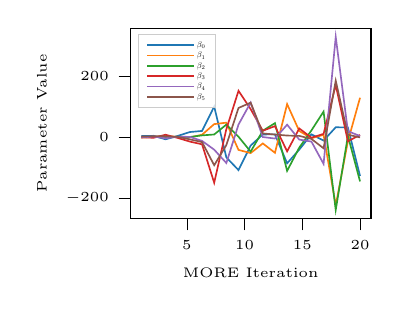
\begin{tikzpicture}

\definecolor{color0}{rgb}{0.12156862745098,0.466666666666667,0.705882352941177}
\definecolor{color1}{rgb}{1,0.498039215686275,0.0549019607843137}
\definecolor{color2}{rgb}{0.172549019607843,0.627450980392157,0.172549019607843}
\definecolor{color3}{rgb}{0.83921568627451,0.152941176470588,0.156862745098039}
\definecolor{color4}{rgb}{0.580392156862745,0.403921568627451,0.741176470588235}
\definecolor{color5}{rgb}{0.549019607843137,0.337254901960784,0.294117647058824}

\begin{axis}[
legend cell align={left},
legend style={
  fill opacity=0.8,
  draw opacity=1,
  text opacity=1,
  at={(0.03,0.97)},
  anchor=north west,
  draw=white!80!black,
  nodes={scale=0.3, transform shape}  
},
tick align=outside,
tick pos=left,
% title={LS unwhitened parameters},
height=4cm,
ticklabel style = {font=\tiny},
xlabel={\tiny MORE Iteration},
ylabel={\tiny Parameter Value},
% ylabel={\tiny parameter value},
x grid style={white!69.0196078431373!black},
xmin=0.105263157894737, xmax=20.9473684210526,
xtick style={color=black},
y grid style={white!69.0196078431373!black},
ymin=-268.197846135806, ymax=356.45825755095,
ytick style={color=black}
]
\addplot [semithick, color0]
table {%
0 nan
1.05263157894737 2.73237046512443
2.10526315789474 3.50329219488935
3.15789473684211 -7.95513196920218
4.21052631578947 3.1963107412616
5.26315789473684 15.9665582377668
6.31578947368421 19.5307936284837
7.36842105263158 99.7682765388784
8.42105263157895 -67.2748857277562
9.47368421052632 -108.935446206743
10.5263157894737 -28.3723498900333
11.5789473684211 8.02737185659973
12.6315789473684 8.25753374056888
13.6842105263158 -86.681775463101
14.7368421052632 -41.7602661650808
15.7894736842105 8.36880712480868
16.8421052631579 -12.0636904267509
17.8947368421053 31.5528074813332
18.9473684210526 30.8502097851426
20 -128.199402412295
};
\addlegendentry{$\beta_0$}
\addplot [semithick, color1]
table {%
0 nan
1.05263157894737 -2.75266552179048
2.10526315789474 -0.222631082543601
3.15789473684211 2.66831225443264
4.21052631578947 0.157081610925826
5.26315789473684 -1.74717757879778
6.31578947368421 7.03076202626305
7.36842105263158 41.8997530423213
8.42105263157895 46.7120202218868
9.47368421052632 -42.7113502411796
10.5263157894737 -53.1940906965109
11.5789473684211 -21.4426407071392
12.6315789473684 -52.1939970742733
13.6842105263158 107.557726652287
14.7368421052632 19.3606919269482
15.7894736842105 -4.40526650509542
16.8421052631579 6.78254399060069
17.8947368421053 -224.674204975011
18.9473684210526 -14.5477576387639
20 128.439447180318
};
\addlegendentry{$\beta_1$}
\addplot [semithick, color2]
table {%
0 nan
1.05263157894737 -0.819022424049623
2.10526315789474 0.199647365891375
3.15789473684211 -1.9428772830007
4.21052631578947 0.500212858929399
5.26315789473684 -0.251013176226387
6.31578947368421 4.9597072663002
7.36842105263158 7.88216971613495
8.42105263157895 40.2859009221452
9.47368421052632 0.532562194060467
10.5263157894737 -48.3780484798251
11.5789473684211 20.277342358223
12.6315789473684 45.129492712781
13.6842105263158 -111.472711995177
14.7368421052632 -35.1344457796991
15.7894736842105 21.2201027003383
16.8421052631579 83.0067829103594
17.8947368421053 -239.804386877317
18.9473684210526 3.34986364357253
20 -145.927381337727
};
\addlegendentry{$\beta_2$}
\addplot [semithick, color3]
table {%
0 nan
1.05263157894737 -0.992314117619856
2.10526315789474 -3.01314990781928
3.15789473684211 6.97978246214006
4.21052631578947 -3.46686242119162
5.26315789473684 -15.4385195979172
6.31578947368421 -24.3729400484366
7.36842105263158 -150.324690640714
8.42105263157895 25.4129175845349
9.47368421052632 151.075076475993
10.5263157894737 91.1111091388412
11.5789473684211 20.0637416066171
12.6315789473684 35.3285999194684
13.6842105263158 -47.4864678609504
14.7368421052632 27.7291529085892
15.7894736842105 -2.6109304150866
16.8421052631579 9.88947690188812
17.8947368421053 170.184421049193
18.9473684210526 -14.380534116013
20 6.50803958125695
};
\addlegendentry{$\beta_3$}
\addplot [semithick, color4]
table {%
0 nan
1.05263157894737 -2.08306644313421
2.10526315789474 1.33198284534283
3.15789473684211 -4.47590681922109
4.21052631578947 0.728904102368964
5.26315789473684 -0.0242990829679821
6.31578947368421 -13.0927089380793
7.36842105263158 -41.9204793443672
8.42105263157895 -85.6876009016413
9.47368421052632 40.4567691407284
10.5263157894737 112.604939441663
11.5789473684211 -0.374362345187074
12.6315789473684 -5.50699678442577
13.6842105263158 40.0725752199367
14.7368421052632 -8.89380637913888
15.7894736842105 -15.351529102298
16.8421052631579 -88.6413918339742
17.8947368421053 328.064798292462
18.9473684210526 18.6842293882621
20 2.86800939663844
};
\addlegendentry{$\beta_4$}
\addplot [semithick, color5]
table {%
0 nan
1.05263157894737 1.06132294724826
2.10526315789474 2.0619373982425
3.15789473684211 1.88073583669649
4.21052631578947 -0.123086282337559
5.26315789473684 -8.07620859625119
6.31578947368421 -17.0593030680154
7.36842105263158 -92.9591020970872
8.42105263157895 -26.8588894445826
9.47368421052632 94.8729166288909
10.5263157894737 112.33820540046
11.5789473684211 11.3158701183703
12.6315789473684 7.71772676655036
13.6842105263158 4.45426808265695
14.7368421052632 3.24805664772185
15.7894736842105 -6.60919932524989
16.8421052631579 -37.4784670914881
17.8947368421053 184.443910566116
18.9473684210526 6.98961781772105
20 -1.46457078349287
};
\addlegendentry{$\beta_5$}
\end{axis}

\end{tikzpicture}
}
  \caption{Example of using LS on 2-dimensional
   Rosenbrock function. The plots show the predicted surrogate model
   parameters $\mathbf{\beta}$. We can see that
   the parameters in whitened space stay in a smaller range 
   making the estimation task easier.}
 \label{fig:whitening}
\end{figure}
  
\subsection{Sample pool}
The original MORE algorithm and other policy search algorithms (REPS)
use a sample pool.
In our approach  we want to avoid using a sample pool and instead use
the information form past samples in the form of the previously predicted
model parameters.

- Still in our experiments the performance better with pool

- talk about doing warm start with no pool

- without pool simply performs worse (but still possible --> maybe
better model noise, prediction parameters)

Idea of increasing the model noise for older samples, encoding the fact that
older samples should have a higher covariance, meaning we are less
certain about them. We implemented this by simple adding a constant
amount to the covariance of the RLS equations for each time a sample is
used. For higher dimensional task this is around 5-10 times.
Still the use of a sample pool is theoretically unsound and problematic,
instead a accurate state transition model could be introduced.
Using the recursive least squares algorithm we had to maintain a sample
pool, because otherwise the resulting estimation was not
satisfactory. From a theoretic perspective this sloppy and ideally we
would refrain from using the sample pool.

We introduced a simple counter for each sample, indicating how many times
the sample has been used.
Then for older samples (higher counter) we increased the model
noise proportionally.
We tried a linear relationship between the counter and
the increased covariance for the model parameters.

$$ new\_cov = constant\_cov\_matrix + w * \text{counter} * \mathbf{I} $$

- TODO: try different weightings: exponential

This improved our results on the rosenbrock test function compared
to the RLS version with constant model noise for all samples.
In each MORE iteration first the oldest samples from the sample pool
are used, meaning the recent samples with lowest model noise are
processed last by RLS.


\subsection{Normalization}
Original MORE approach uses standard score normalization, doing it
in a batch way at each iteration for all samples in the sample pool.

different ways of normalization:

- exponential weighting (search for citation)

- standard score

\section{MORE with Recursive Surrogate-Modeling}
\begin{algorithm}[H]

\DontPrintSemicolon
\SetAlgoLined
\KwIn{Parameters $\epsilon$ and $\beta$, \\ $K$ number of iterations, $N$ samples per iteration}
\Begin{Initialization:}
{
  Initialize search distribution $\pi$
  Initialize RLS$(\mathbf{m}_0, \mathbf{P}_0)$
}
\For{$k = 1,...,K$}
{
  \For{$n = 1,...,N$}
  {
    Draw parameters $\theta_n \sim \pi$\;
    Execute task with $\theta_n$ and receive $R(\theta_n)$\;
  }
  \Begin(Estimate quadratic model)
  {
    \For{$n = 1,...,N$}
    {
      Whitening: $\mathbf{W}\phi(\mathbf{\theta}_n)$\;
      Optionally: Use normalization\;
      Optionally: Increase model noise for older samples\;      
      compute surrogate model parameters with RLS  \cref{RLS:basic}\;
    }
  }
  Solve  $\text{argmin}_{\eta >0, \omega > 0} \, g(\eta, \omega)$
  using \Cref{eq:dual} \;
  Update search distribution $\pi$ using \Cref{policy_update}\;
}
\caption{MORE Algorithm with Recursive Surrogate-Modeling}
\end{algorithm}



%\subsection{Moving back to prior}
%One technique we investigated is 
%- to prior calculation (optimal for whitened space)
%
%- set up equation
%
%\subsection{State Transition Model}
%Let us quickly state the full Kalman filter equations, the
%derivation can be found in the appendix (TODO ref)
%
%Prediction step:
%
%Update step:
%
%Introducing an accurate state transition model to incorporate the
%prediction step of the kalman filter would be ideal.
%We tried some simple momentum approaches based on the differences of
%subsequent surrogate model parameters, but those did not yield
%good results.
%Our Recursive least squares algorithm is a special case of these
%equations using an state transition model matrix $\mathbf{A} = \mathbf{I}$.
%